\documentclass[a4paper, 12pt]{article}

\usepackage[T1]{fontenc}
\usepackage[utf8]{inputenc}
\usepackage[english]{babel}  % ngerman for German
\usepackage{lmodern}  % nicer font
\usepackage{geometry}
\geometry{%
	left   = 2.5cm,
	right  = 2.5cm,
	top    = 3cm,
	bottom = 3cm
}

\usepackage{textcomp}
\usepackage{gensymb}
\usepackage{amsmath,amssymb,amsfonts}
\usepackage{nicefrac}  % nicer inline fractions
\usepackage{tensor}  % allows fancy indices
\usepackage{siunitx}  % easy handling of value + unit (e.g. \SI{10}{\pF})
% \sisetup{}  % configure siunitx (e.g. locale = DE)
\sisetup{output-complex-root=\ensuremath{\mathrm{j}}, complex-root-position = before-number} % configures SI format 10 + j5 for complex numbers (instead of 10 + 5i)

\usepackage{listings}  % code listings
\usepackage{enumerate}
\usepackage{booktabs}  % nicer tables (e.g. \toprule)
\usepackage{verbatim}  % inline code (\verb||)
\usepackage{subcaption}  % captions for subplots
\usepackage[european, siunitx, RPvoltages]{circuitikz}  % draw circuit diagrams
\usepackage{enumitem}
\setlist[itemize]{label=\rule[0.5ex]{0.6ex}{0.6ex}} % black squares for itemize

\usepackage{pstool}  %% Tex fonts in EPS files
\usepackage{graphicx}
\graphicspath{{./figures/}}

\usepackage{etoolbox} % Needed for AtBeginEnvironment command (appendix handling)
\usepackage{appendix} % Appendices environment

\usepackage{csquotes} % removes biber warning
\usepackage[  % ieee style citations (e.g. [1])
	backend     = biber,
	maxbibnames = 99,
	autocite    = footnote,
	style	    = ieee,
	citestyle   = numeric-comp,
	doi=false, isbn=false
]{biblatex}
\addbibresource{bibliography/bibliography.bib}

\usepackage[nobiblatex]{xurl}  % line breaks in URLs
% last imports
\usepackage[bookmarksopen,colorlinks,citecolor=black,linkcolor=black, urlcolor = black]{hyperref}

% after hyperref! 
\usepackage[noabbrev, nameinlink]{cleveref} 
% e.g. \cref{label} or \Cref(label) for capital letter
% configure cleveref not to use brackets around equation references
\creflabelformat{equation}{#2\textup{#1}#3} % Equation references without parentheses
\AtBeginEnvironment{appendices}{\crefalias{section}{appendix}} % Appendix referencing (for cref "Appendix A" instead of "Section A")


% add missing hyphenations
\hyphenation{im-ple-men-ta-tions}

\title{ECS7012P - Music and Audio Programming\\
	   Final project: Pitch detection}
\author{
  Max Tamussino, 200579179
}
\date{\today}


\begin{document}

\maketitle
\tableofcontents
\pagebreak

% \begin{figure}[h!]
% 	\centering
% 	\includegraphics[width=\textwidth]{}
% 	\caption{}
% 	\label{fig:}
% \end{figure}

\section{Introduction} \label{sec:intro}
This report covers the design and implementation of a simple pitch detection device using the Bela Platform \cite{McPherson2015}. The frequency content of a pre-recorded file or of live microphone input is analysed using the fast fourier-transform (FFT) and the fundamental frequency is detected. A browser-based graphical user-interface (GUI) is used to present the calculated spectrum and show the detection result. Additionally, for the possible application of tuning instruments, useful information for tuning is shown. The spectrum graph axis may be edited by provided settings.


\section{Background}
There are many algorithms to detect the pitch of a signal. Most of these use the so-called autocorrelation function \cite{Amado2008}, less sophisticated methods just utilise the fourier transformation. Both mathematical concepts are briefly summarised.

\subsection{Autocorrelation}
The autocorrelation function (ACF) of any time-continuous real signal $x(t)$ is defined as the cross correlation with itself \cite{Rao2020} at lag $\tau$, as given in \Cref{eq:autocorr-c}. Qualitatively, the value of the ACF is proportional to the degree of similarity \cite{Apicella2013} between the signal and itself shifted by lag $\tau$.

\begin{equation}
	\label{eq:autocorr-c}
	r_x(\tau) = \int_{-\infty}^{\infty} x(t) \cdot x(t + \tau) \, dt
\end{equation}

The ACF shows a global maximum at $r_x(0)$ and local maxima at lags $\tau$ which correspond to the time period $P$ of a frequency component of $x(t)$ \cite{Rabiner1977,Staudacher2016}. To be able to set static thresholds, the normalised ACF $r_x'(\tau) = r_x(\tau) / r_x(0)$ $P$ may then be used to calculate the dominant frequency $f_0=1/P$ of the given signal. In the case of sampled discrete-time signals, which are given as blocks of finite length $N$, the autocorrelation is given in \Cref{eq:autocorr-d}.

\begin{equation}
	\label{eq:autocorr-d}
	r_x[k] = \sum_{n=0}^{N-1} x[n + k] \cdot x[n]
\end{equation}

\subsection{Fourier transformation}
The fourier transformation (FT) decomposes signals into their individual frequency components. The mathematical form of this integral transformation and its inverse (iFT) for continuous-time signals $x(t)$ is given in \Cref{eq:fourier-c}.

\begin{align}
	\label{eq:fourier-c}
	X(f) = \int_{-\infty}^{\infty} x(t) \cdot e^{-j 2\pi ft} \, dt && 
	x(t) = \int_{-\infty}^{\infty} X(f) \cdot e^{j 2\pi ft} \, dt
\end{align}

The power spectral density $S_x(f)$ may then be extracted from the magnitude of $X(f)$ by $S_x(f) = |X(f)|^2 = X(f) \cdot X^*(f)$. The discrete-time equivalent of the fourier transformation (again for finite blocks with length $N$ of sampled data), often called the DFT, is given in \Cref{eq:fourier-d}. The DFT yields exactly $N$ unique frequency \emph{bins} (for real signals actually only $N/2$ bins are unique), where each index $k$ korresponds to a certain frequency $f_k=k \cdot \Delta f$ of the originally continuous sampled signal $x(t)$, where $\Delta f = f_s/N$ and $f_s$ is the sampling frequency. This statisfies the nyquist criterion, as for real signals sampled with $f_s$, only frequencies up to $f_s/2$ can be resolved.

\begin{align}
	\label{eq:fourier-d}
	X[k] = \sum_{n=0}^{N-1} x[n] \cdot e^{-j 2\pi \frac{n}{N} k} &&
	x[n] = \frac{1}{N} \cdot \sum_{n=0}^{N-1} F[k] \cdot e^{j 2\pi \frac{n}{N} k}
\end{align}

There are very efficient implementations of the DFT for block sizes $N=2^n$. These fast implementations are referred to as fast fourier transform or FFT and are complexity order $O(N \log N)$ instead of the orginal FT with $O(N^2)$. Because of these, the ACF for large block sizes is often calculated by using the Wiener-Khintchine Theorem $r_x(\tau)= iFFT \left[ S_x(f) \right]$ \cite{Apicella2013}.


\section{Design}
The method used in this project primarily uses the obtained spectrum of the FFT to detect and calculate the fundamental frequency also referred to as \emph{spectral peak picking} \cite{Knesebeck2010}.

\subsection{Input}
The input signal is either sampled from a microphone or retrieved from recordings. The latter relies on sound files recorded with a sampling rate of $f_s=\SI{44.1}{\kilo\hertz}$, as the same is used for live microphone input. In the case of live input, a simple electret microphone is connected to one of the Bela audio input channels as shown in \Cref{fig:mic-wiring}. The input method can be switched by pressing a button, which is located on the same breadboard as the microphone.

\begin{figure}[h!]
	\centering
	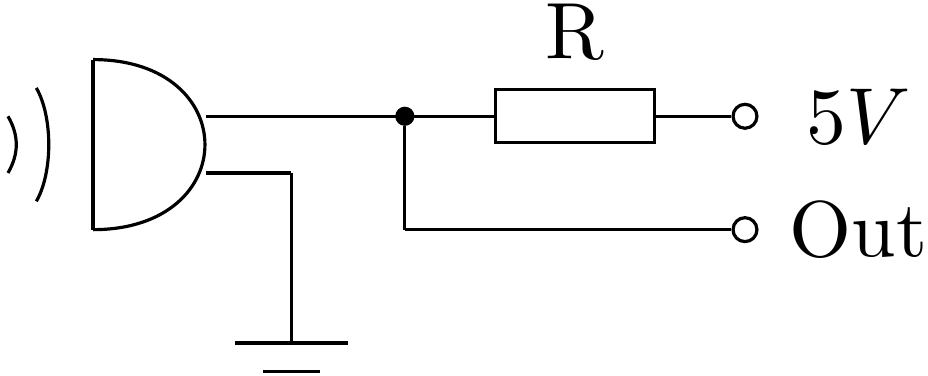
\includegraphics[width=0.3\textwidth]{mic-wiring.png}
	\caption{Wiring for the used electret microphone with $R=\SI{10}{\kilo\ohm}$}
	\label{fig:mic-wiring}
\end{figure}

\subsection{Downsampling}
As mentioned previously, a standard sampling rate of $f_s=\SI{44.1}{\kilo\hertz}$ is used initially. For the block-based processing of this data, overlapping windows of length $N=2048$ and a hop size of $512$ were chosen. Applying the FFT directly to one window with $f_s$ would resolve frequencies up to $f_{max}=f_s/2=\SI{22.05}{\kilo\hertz}$. However, the frequency resolution calculates to $\Delta f=f_s/N=\SI{21.5}{\hertz}$, which is unacceptable for tuning instruments. A higher resolution could be reached by increasing $N$, however this is not feasible considering the amount of time these calculations would take for each window. The resolution was instead increased by downsampling the input signal by a factor of $16$. This greatly improves frequency resolution to $\Delta f=f_s/(16 \cdot N) =\SI{1.35}{\hertz}$. On the other hand, it leads to a significantly decreased maximum detectable frequency of $f_{max}=f_s/32=\SI{1.38}{\kilo\hertz}$, which is however sufficient for most instruments.

\subsection{Maximum detection and fundamental check}
If a full window of $N=2048$ samples is assembled, the FFT is calculated. From the FFT, the discrete spectrum magnitude $S_x[k]$ is obtained and its maximum value detected. For some instruments however, the fundamental frequency is not the global maximum of the spectrum. Especially guitars often show the global maximum at the second or third harmonic \cite{Knesebeck2010}. This is why after the global maximum at the dominant frequency $f_d$ is found, the regions at one half and one third of $f_d$ are examined. Should one of these local maxima exceed \SI{70}{\percent} of the global maximum, it is considered that $f_d$ is a harmonic of the fundamental frequency $f_0$. Otherwise, the dominant frequency is considered to be equal to the fundamental frequency.

\subsection{Interpolation}
The previously determined local maximum in the spectrum may be further refined. Because the maximum of the continuous spectrum is most likely not to coincide with the center of the frequency bin, parabolic interpolation as proposed in \cite{Gasior2004} is used to improve the FFTs accuracy beyond $\Delta f$. Using the two neighbour values to the local spectrum maximum, parabolic interpolation is performed by calculating the non-integer frequency index $k' = k_{max} + \Delta_k$ by \Cref{eq:interpol}, which can then be used to calculate the refined frequency $f_0= \Delta f \cdot k'$.

\begin{equation}
	\label{eq:interpol}
	\Delta_k = \frac{S_x[k_{max}+1] - S_x[k_{max}-1]}{2 \cdot (2 \cdot S_x[k_{max}] - S_x[k_{max}+1] - S_x[k_{max}-1])}
\end{equation}

\subsection{User Interface} \label{sec:gui}
The user interface is displayed in the browser of a connected PC, as depicted in \Cref{fig:gui-all}. The spectrum of the given input is displayed in the graph, which also indicates where the current fundamental is detected by a vertical line. Below, both frequency and magnitude axis of the graph may be edited using the settings. Minimum, maximum and the label steps may be changed in the textboxes, pressing \emph{Set} will then apply these changes. Pressing \emph{Reset} will put the graph in its default state. Additionally, by pressing \emph{Pause/Resume}, the graph may be stopped to have a closer look at the spectrum while the axis settings still are modifiable. Next to the settings, the results are presented - the fundamental frequency and its corresponding MIDI standard note number.

At the bottom right of \Cref{fig:gui-all}, the instrument tuning information is shown. The measured fundamental frequency will generally not perfectly match one note. In this case, the bar at the bottom will move out of its center. Should the instrument be far from calibrated, the bar moves in yellow and red areas respectively. The nearest note is usually the tuning goal and is achieved when the bar moves directly into the center. Using english notation, the nearest note is therefore written above the center of the tuning bar. The next and previous notes are given at the sides.

\begin{figure}[h!]
	\centering
	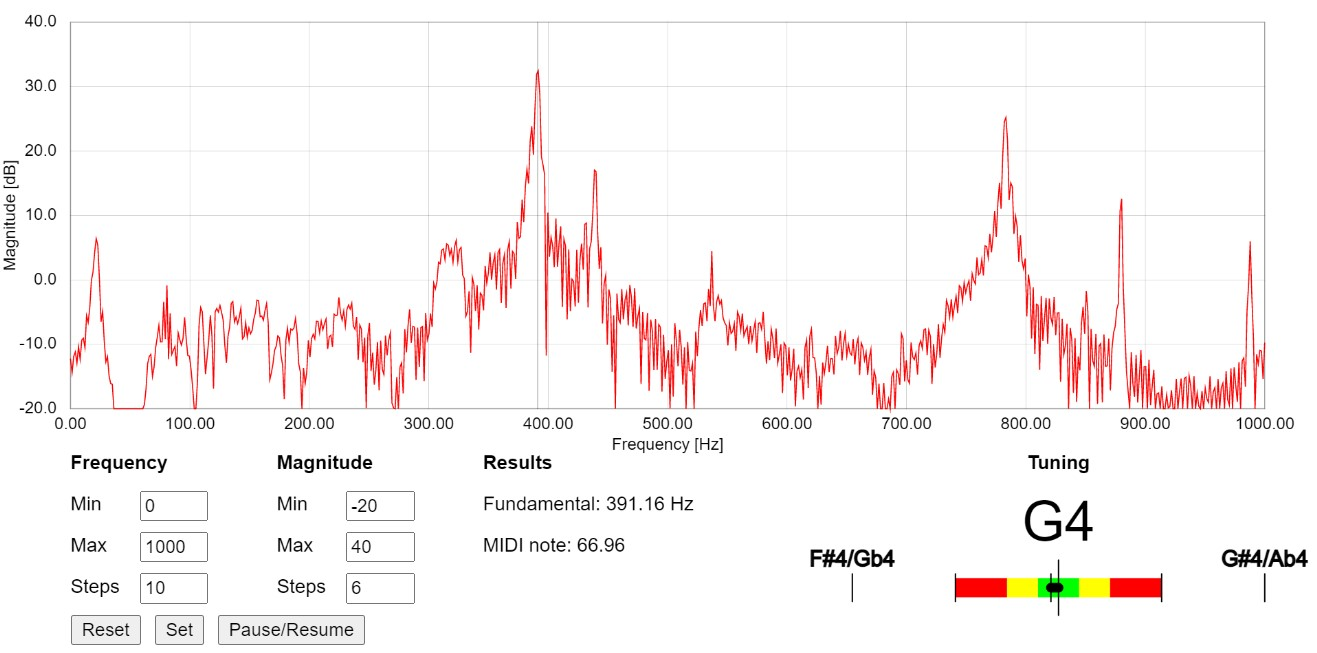
\includegraphics[width=\textwidth]{gui-all.jpg}
	\caption{The browser-based GUI with spectrum graph, axis settings, results and instrument tuning information}
	\label{fig:gui-all}
\end{figure}

\section{Evaluation}
The device was only tested using a reference tone generator, no real instrument was available. For every tested reference frequency, the device showed an error lower than \SI{0.1}{\percent}. However, it must be said that the only noise present was a peak at \SI{50}{\hertz}, which was most likely due to the power connection of the microphone showing grid frequency. Recordings of pianos and guitars were tested and yielded the correct notes, however the tuning of these instruments is not known and the slight detuning which was measured could originate both in an error of the designed device or the actual instrument.

String instruments, like the guitar, which show stronger harmonics than fundamental frequencies in their spectrum, are considered to be the weakness of the spectrum peak-picking method. Allthough the wrong detection of second and third harmonics as fundamental frequencies was circumvented, the design is will certainly encounter difficulties with instruments that were not tested. Other approaches using the autocorrelation function could yield better results for those instruments. However, calculating the FFT twice is computationally highly expensive and did not yield statisfying image refresh rates for the GUI in this project. The PRAAT pitch detection algorithm proposed in \cite{Boersma93} using advanced autocorrelation techniques would be an interesting alternative.

Additionally, other methons of picking up the instruments sound could be used. Mechanical vibrations, for example, could be measured with an accelerometer. This approach would yield better results in noisy environments, as acoustic noise would not interfere with measurements.

\clearpage
\sloppy
\printbibliography

\end{document}